\cleardoublepage
\chapter{Implementation and Evaluation}
\label{chapter:evaluation}

We now offer an evaluation that attempts to explore the overhead of the stronger consistency model of fastPSI, compared to the weakest consistency model that satisfies the atomicity of transactions, namely Read Committed. We also show how fastPSI is able to outperform a protocol implementing the stronger Serialisability consistency model. Finally, we evaluate the scalability of fastPSI as more servers and partitions are added to the system, and discuss some of the weak points of the protocol.\todonote{rephrase?}

\section{Implementation}

Our implementation of the fastPSI protocol consists of a client-side library~\citep{pvc-client} and a server~\citep{pvc-server}, the latter being written as a plug-in transactional protocol for Antidote~\citep{antidote-db}, a reference platform for evaluating consistency protocols. Both the client library and the server are written in the Erlang programming language, with a total of 6K lines of code. The Antidote platform provides a key-value database, supports both in-memory and disk-based storage, and implements full replication. For simplicity, our implementation only supports in-memory storage, and lacks a replication mechanism. The client-side library communicates with the server using Google's Protocol Buffers~\citep{protobuf}. To enhance network efficiency, client messages are transmitted in periodic batches to the servers.

To validate the results of our evaluation, we also implement two alternative protocols satisfying the Read Committed and Serialisability consistency models, called \textbf{naiveRC} and \textbf{naiveSER}, respectively. Both are built on top of our original implementation and are as efficient as possible. The pseudocode for both implementations can be found in Appendix~\ref{appendix:code}.

Given that fastPSI requires the use of multiple versions per object, it becomes necessary to prevent an unbounded growth of the number of versions in the $\VersionLog$ database, and in the number of entries in the per-partition $\CommitLog$. We implement a simple garbage collection mechanism that maintains a fixed number of versions and that regularly prunes the oldest versions from the state of a partition.\todonote{Mention tradeoff w/ number of versions and abort ratio?}

\section{Evaluation}

We evaluate the performance of fastPSI using the Yahoo! Cloud Serving Benchmark~\citep{ycsb}, modified to generate transactional workloads~\citep{ardekani_nmsi, ardekani_gdur}. Our implementation of Read Committed is used as a baseline for comparison, in order to show the maximum possible performance. Figure~\ref{fig:workload-types} describes the workloads used\todonote{mention that D and E are invented. Maybe say that we take inspiration from YCSB, instead of saying that we use it}. All experiments are run on a cluster consisting of machines running Debian 4.19.67-2 (Stretch) with 3.80~GHz to 4.70~GHz Intel Xeon processors with six cores, 32~GB of RAM, and a single 1~Gbps network port. We partition the cluster in up to three different sites, with four server machines and four client machines in each site. Thus, there is no shared memory between clients and servers, as if clients were acting as proxies in the same data centre as servers. Since all our machines are located in the same local network, we artificially add latency between sites using the \texttt{tc} Linux command.

In all our benchmarks, the system is loaded with one million random keys and 256-byte values prior to receiving any operations from the clients. Partitions are distributed uniformly across servers, such that a server might be responsible for multiple partitions. Keys are mapped to partitions using consistent hashing, with clients being aware of the distribution of keys to partitions and server machines. Thus, clients can directly address the correct server and partition for a specific key. Each client machine spawns multiple concurrent threads that execute transactions and communicate with servers in a closed-loop fashion. When transactions read more than object, clients perform those operations serially. For the experiments that involve more than one site, the latency between sites is of 10~ms.

\begin{figure}[h]
\begin{center}
\begin{tabularx}{0.85\linewidth}{ c | c | >{\centering}X | >{\centering}X }
    & \multirow{2}{*}{Key Selection Distribution}
    & \multicolumn{2}{c}{Operations}
\tabularnewline
    & & Read-Only Tran.
    & Update Tran.
\tabularnewline
    \hline
    % A & Zipfian & 4 Reads & 2 Reads, 2 Updates \tabularnewline
    B & Uniform & 4 Reads & 3 Reads, 1 Update \tabularnewline
    C & Uniform & 2 Reads & 1 Read, 1 Update \tabularnewline
    D & Uniform & 3 Reads & 3 Reads, 1 Update \tabularnewline
    E & Uniform & 3 Reads & 3 Reads, 3 Updates \tabularnewline
\end{tabularx}
\end{center}
\caption{Transactional YCSB Workload Types.}
\label{fig:workload-types}
\end{figure}

\subsection{Performance \& Scalability Limits}

\paragraph{Performance.} We begin by investigating the overall performance profile of our implementations. We measure and compare the throughput and latency of the different protocols as the number of update transactions increases, while keeping the number of sites constant. For this experiment, we vary the number of concurrent client threads such that we never saturate the CPU of servers. We aim to explore the overall overhead of fastPSI in comparison with naiveRC, as well as the performance benefits it offers in comparison with naiveSER. Figure~\ref{fig:general_bench} shows the results of using Workload C and three sites, with 64 partitions uniformly distributed across sites. We vary the ratio of read-only to update transactions, from 90\%/10\% to 70\%/30\% (left to right), and measure the termination latency of update transactions, i.e., the amount of time spent on the validation process of a transaction. Since the latency is measured in the client, it only reflects the amount of time spent on the \emph{prepare} phase of the commit validation, as the client does not need to wait until the changes of a transaction are committed to the partition state.

\begin{figure}[t]
\vspace{-0.5cm}
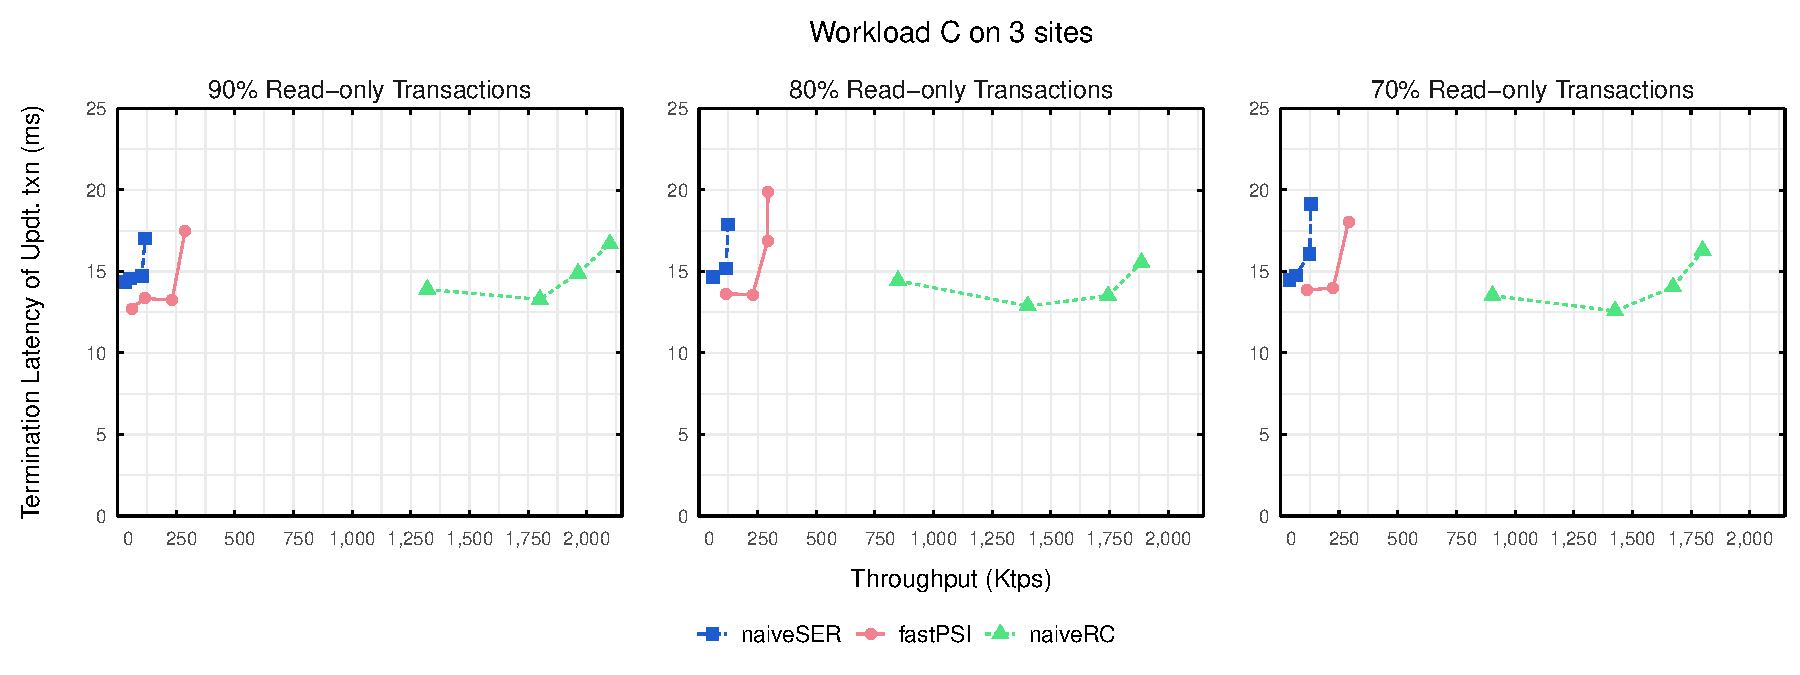
\includegraphics[width=\textwidth]{figures/general_bench.pdf}
\vspace{-1cm}
\caption{Comparison of throughput and termination latency of update transactions. \todo{Move legend to top, remove title?}}
\label{fig:general_bench}
\end{figure}

Transactions as executed by naiveRC need minimal synchronisation during its commit phase, and no synchronisation at all during read operations. This is reflected in its high performance, with the validation of update transactions as the only bottleneck in the system. Thus, as the proportion of update transactions increases, the impact on overall throughput is pronounced, dropping by as much as 20\%.

For both naiveSER and fastPSI, read operations from a transaction $\tx$ must wait until the causal dependencies of $\tx$ commit at a particular partition, bounded in the worst case by the maximum latency across sites. In addition, read operations accessing the same partition suffer from having to synchronise while fixing a snapshot, as the implementation of $\CommitLog$ is not thread-safe. These two shortcomings explain the overall low throughput in comparison with naiveRC. Nevertheless, both implementations exhibit stable performance as the proportion of update transactions increases.

By comparing fastPSI with naiveSER, we observe that the latter implementation is limited by its need to validate every transaction, in comparison with fastPSI, which only validates update transactions. In addition, the weaker consistency model offered by fastPSI allows it to outperform naiveSER in all cases by approximately 150\%, while showing similar latencies.

\paragraph{Scalability.} To explore the overall scalability of fastPSI, we examine how the maximum performance of each protocol changes as we increase the number of machines in the system. We use Workload B with a fixed ratio of 10\% update transactions, and vary the number of sites from one to three, while keeping the number of partitions fixed to 64. Figure~\ref{fig:site_bench} shows the overall performance of the protocols.

\begin{figure}[h]
\begin{center}
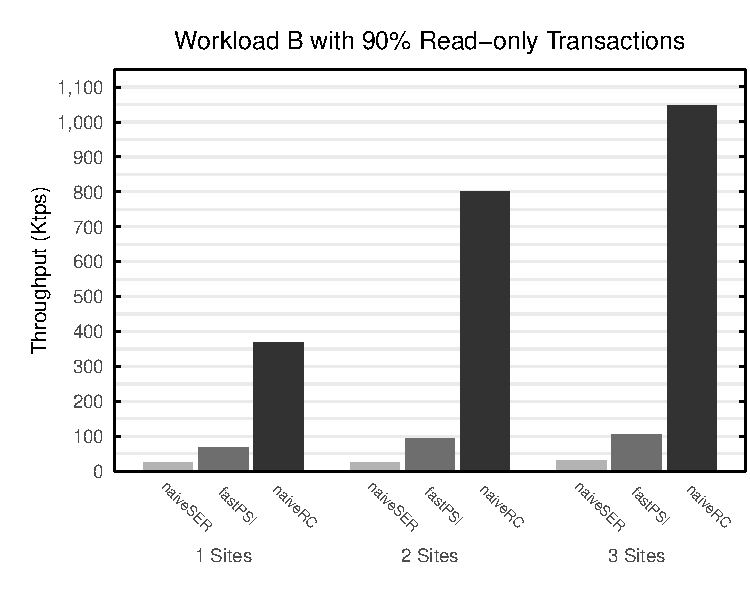
\includegraphics[width=0.5\textwidth]{figures/sites_bench.pdf}
\vspace{-1cm}
\end{center}
\caption{Maximum Throughput of Consistency Models.}
\label{fig:site_bench}
\end{figure}

As before, the performance of naiveRC increases almost in a linear fashion as we add more servers, as explained by its minimum need for synchronisation. Although the scalability of fastPSI is limited by the fixed number of partitions, it benefits moderately from increasing the number of machines: as the overall number of partitions per machine decreases, servers free resources, and can thus fulfil more client requests. This is reflected in its performance at three sites being 1.52 times its base throughput at a single site. In contrast, the overall performance of naiveSER stays almost constant as we increase the number of sites, reflecting its need to validate every transaction, which requires greater levels of synchronisation as the number of machines increases.

As the number of sites increases, so does the difference between naiveSER and fastPSI. Overall, fastPSI manages to outperform naiveSER by a factor of 2.88 with a single site, and by a factor of 3.52 at three sites.

\begin{figure}[h]
\begin{center}
\begin{tabularx}{0.75\linewidth}{ l | >{\centering}p{5cm} | >{\centering}X }
   \textbf{Parameter} &\textbf{Range} &\textbf{Default}
\tabularnewline
    \hline
    Sites & 1--3 & 3
\tabularnewline
    Update Tran. Proportion & 10\%--30\% & 10\%
\tabularnewline
\end{tabularx}
\end{center}
\vspace{-0.5cm}
\caption{Parameter space used in the comparison workload.}
\label{fig:dynamic_parameters}
\end{figure}

\begin{figure}[t]
\begin{center}
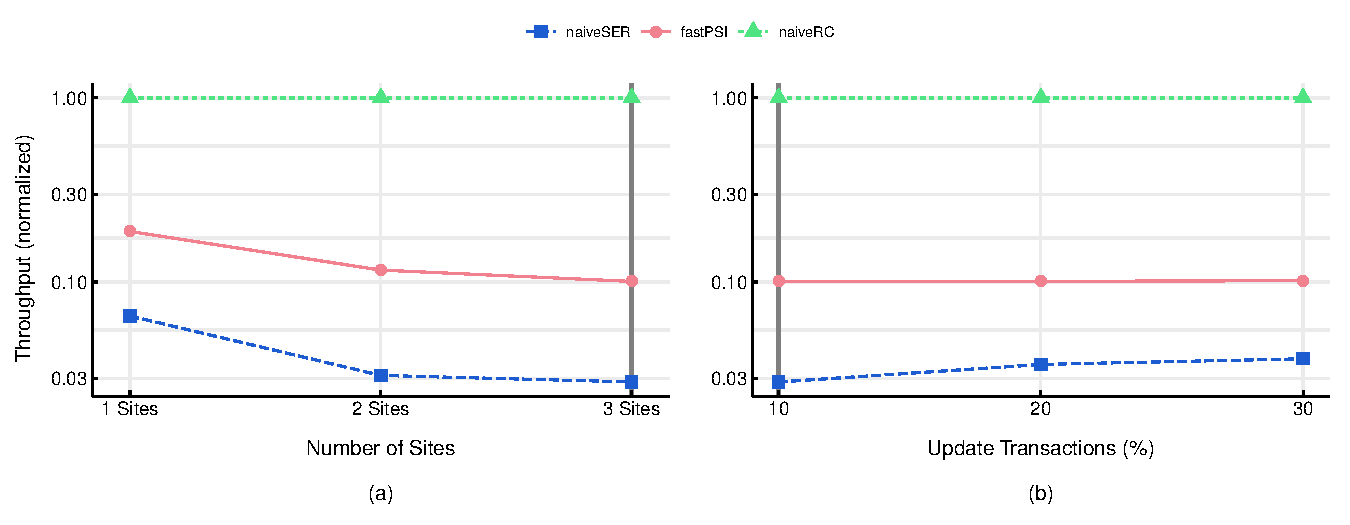
\includegraphics[width=0.8\textwidth]{figures/dynamic_bench.pdf}
\vspace{-0.75cm}
\end{center}
\caption{Parameter space exploration to reflect the performance comparison of the protocols. Each experiment varies one parameter while keeping the other fixed at its default value (represented by the grey vertical line). Throughput is shown normalised compared to naiveRC.}
\label{fig:dynamic_bench}
\end{figure}

\paragraph{Overall comparison.} We've seen how the performance and scalability of the implementations is determined by the proportion of update transactions and the number of sites. To better visualise the relationship between workload choice and performance, we explore the parameter space described in Figure~\ref{fig:dynamic_parameters} when using Workload B. As in the previous experiment, we keep the number of partitions constant as we increase the number of sites. The results are shown in Figure~\ref{fig:dynamic_bench}, with the throughput depicted normalised compared to the performance of naiveRC.

As shown in Figure~\ref{fig:dynamic_bench}a, fastPSI and naiveSER have different scalability properties. Although both implementations suffer in comparison with naiveRC, fastPSI exhibits much better scalability in comparison with naiveSER. For naiveSER, the need to validate every transaction imposes a performance penalty that increases as we add more sites, and consequently increases the overall latency of the commit phase for every transaction. In contrast, the impact on fastPSI is less severe, as the increased latency only affects the read operations, since the proportion of update transactions is low.

Figure~\ref{fig:dynamic_bench}b shows the performance comparison as the proportion of update transactions increases. While the difference in throughput between naiveRC and fastPSI stays constant, the overall performance of fastPSI is hindered by the need to compute a causally compatible snapshot. Nevertheless, the fact that the relative performance stays constant in comparison with naiveRC shows that the impact of the validation process does not grow with the number of update transactions. The impact of update transactions on naiveSER is less pronounced, and its performance difference with fastPSI gets smaller as the proportion of updates increases. This is explained by the choice of workload: read-only transactions perform four reads, while update transactions perform three. Since naiveSER also validates read-only transactions, as the proportion of update transactions grows, the average number of partitions that participate in the voting phase shrinks from four to three, which decreases the runtime cost of validation.

\subsection{Abort Ratio}
\label{subsect:abort_ratio}

We now focus on another advantage of the relaxed consistency model of fastPSI in comparison with serialisability, namely, the ratio of aborted transactions. One of the advantages of fastPSI is that the snapshots of transactions exhibit \emph{forward freshness}: a transaction $\tx$ is able to read object versions written by transactions that committed after $\tx$ started. In contrast, a transaction $\tx$ under Serialisability or classical Snapshot Isolation can only read versions written by transactions that commit before $\tx$'s start time. This limitation leads to a high number of aborted transactions in high latency settings, due to stale reads.

\begin{figure}[t]
\begin{center}
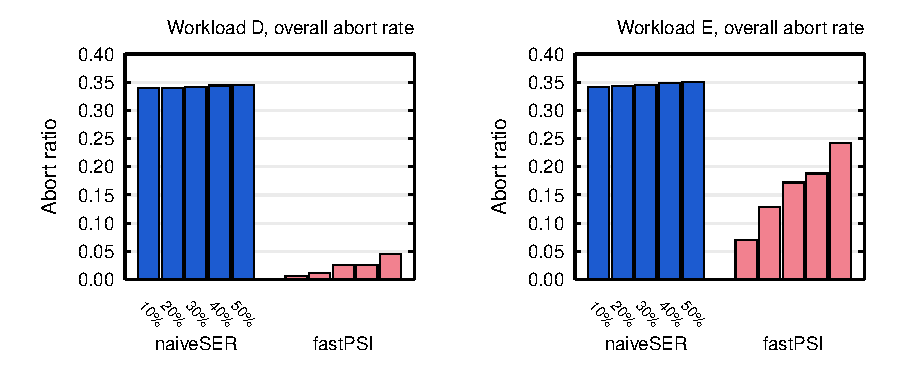
\includegraphics[width=0.8\textwidth]{figures/abort_rate_bench_overall.pdf}
\vspace{-0.75cm}
\end{center}
\caption{Overall transaction abort ratio for different consistency models and workloads.}
\label{fig:raw_abort_rate_overall}
\end{figure}

In this section, we aim to explore the advantages of forward freshness in fastPSI in comparison with naiveSER, and how different workloads affect it. In Figure~\ref{fig:raw_abort_rate_overall}, we show how the abort ratio of transactions varies---under different workloads---with the number of update transactions. The results were obtained with two sites. The graph on the left shows the advantages of the forward freshness of transactions, with the abort ratio of fastPSI being 30 percentage points better than naiveSER, on average. However, as the number of update transactions increases, so does the number of conflicting transactions. This is reflected in an increase of aborted transactions, from less than one percent to around five percent. The graph on the right, however, shows different results: as the number of update transactions grows, so does the overall abort ratio of fastPSI, from 7\% to 25\%. Overall, in the worst case the abort ratio of fastPSI is only 10 percentage points better than naiveSER.

To understand the difference between workloads, we turn to the two graphs depicted in Figure~\ref{fig:raw_abort_rate_2pc}, which explore the reasons why transactions abort. In fastPSI, a transaction might abort for two reasons: by updating an object that is overwritten by a concurrent transaction, or by failing to form a causally consistent snapshot, as detailed in~\ref{sect:read_aborts}. By virtue of having the same implementation of causally consistent snapshots, naiveSER inherits the same reasons, and adds a third: if a transaction reads a version of an object that is later overwritten, it is forced to abort. For both protocols, we say that a transaction might abort at two points during its execution: read aborts occur when a transaction fails to fix a causally consistent snapshot, and otherwise we say that the transaction aborts during validation, i.e., during the termination of the transaction. On the left, we see that for Workload D, all aborted transactions in fastPSI do so during the validation phase, while for naiveSER, only a small percentage of aborted transactions (between 0.5\% and 2.5\%) do so during termination. In contrast, fastPSI exhibits a very different behaviour with Workload E, as shown in the graph on the right. With this workload, transactions abort for the same reason in both protocols: they are unable to build causally consistent snapshots. In both cases, the amount of transactions that abort while attempting to fix a snapshot grows as the number of update transactions increases.

\begin{figure}[t]
\begin{center}
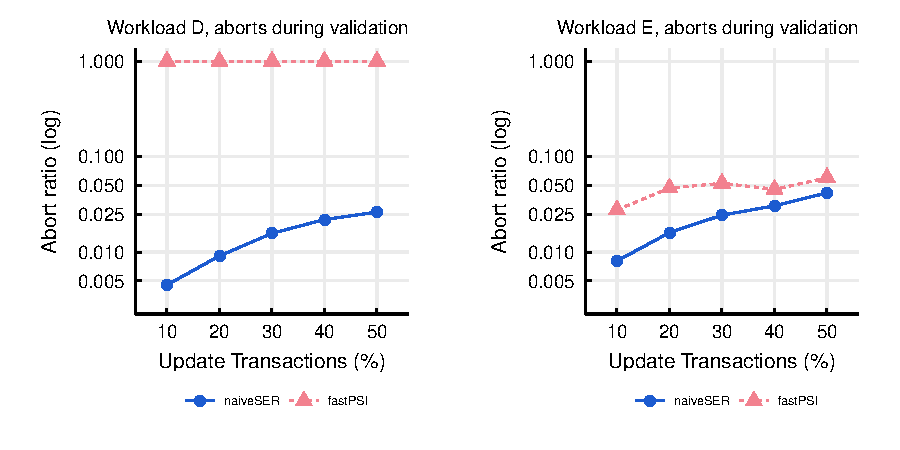
\includegraphics[width=0.8\textwidth]{figures/abort_rate_bench_2pc.pdf}
\vspace{-0.75cm}
\end{center}
\caption{Ratio of aborts that happen during the validation phase, for different consistency models and workloads.}
\label{fig:raw_abort_rate_2pc}
\end{figure}

Recall that in Workload D, update transactions update one single key, while in Workload E, they update three. This small difference in the number of update keys explains the difference in aborted transactions for fastPSI. As described in~\ref{sect:read_aborts}, a transaction $\tx$ will be unable to fix a causally consistent snapshot when a) different partitions commit non-conflicting transactions in different order, and b) $\tx$ fixes a snapshot in one of those partitions before the updates of all the non-conflicting transactions become visible. Since update transactions in Workload D only update a single key, update transactions will only commit at a single partition, and therefore, no transaction can observe a different commit order. This explains why there are no aborted transactions due to inconsistent snapshots when executing this workload for fastPSI. In contrast, update transactions in Workload E update three keys, and therefore commit at three different partitions,\footnote{Since transactions choose keys following an uniform distribution, most keys will be managed by distinct partitions.} such that the probability of partitions committing transactions in different order grows. In addition, since transactions read three keys, the probability of observing different commit orders also grows. Thus, as we increase the number of update transactions, so does the probability of transactions attempting to fix inconsistent snapshots. In naiveSER transactions also commit at the partitions they read from, meaning that update transactions in Workload D commit at three partitions. This explains why its abort ratio of  is similar in both workloads.

\begin{figure}[t]
\begin{center}
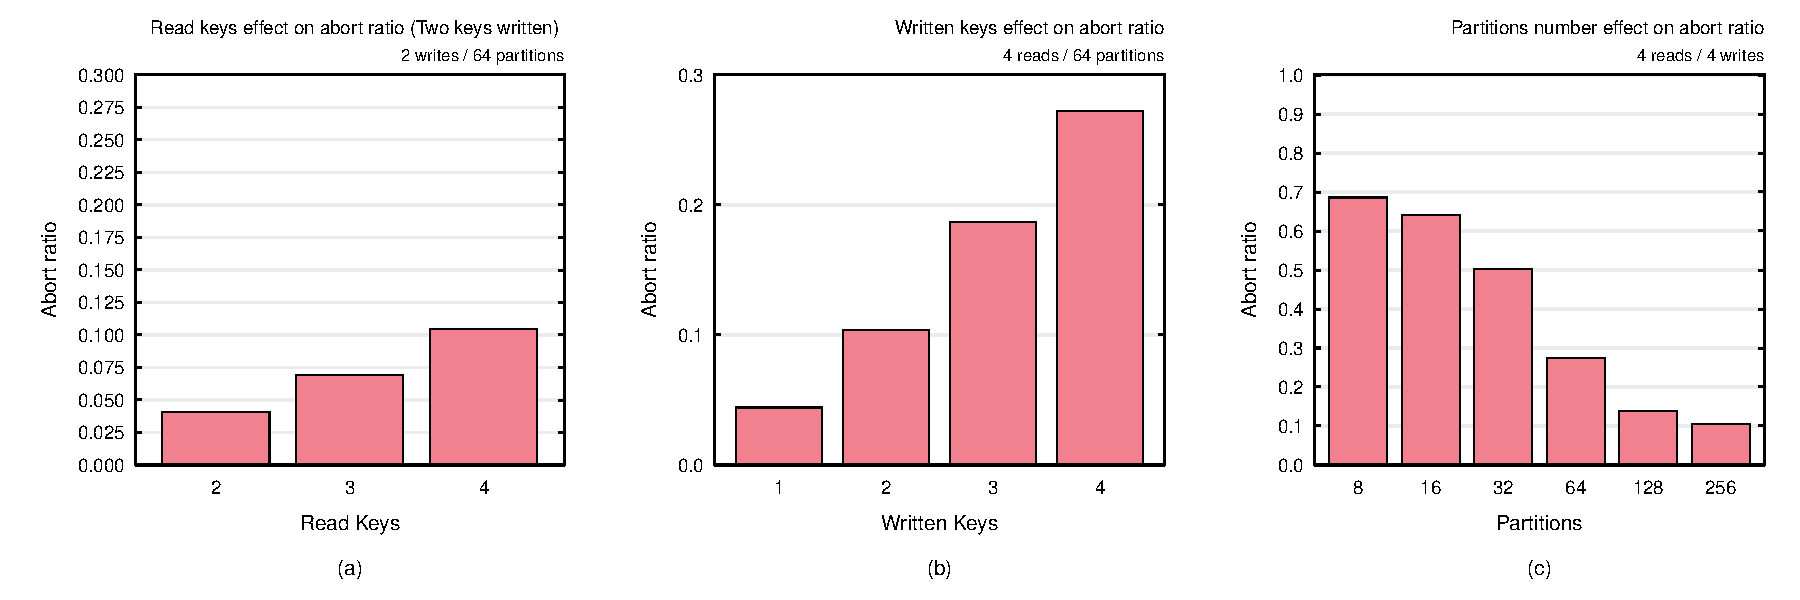
\includegraphics[width=\textwidth]{figures/psi_read_abort_bench.pdf}
\vspace{-1cm}
\end{center}
\caption{Results from exploring the abort rate of fastPSI across different workload and deployment scenarios.}
\label{fig:fastpsi_abort_rate}
\end{figure}

Since small changes in workload choice are able to affect the overall abort ratio of fastPSI in a significant manner, we finish our evaluation with an exploration of the parameters that have the highest impact on the number of aborted transactions. As explained previously, one of the reasons why transactions observe inconsistent snapshots is because partitions commit transactions in different orders. Thus, by changing the number of keys updated by a transaction, we can modify the number of partitions involved, which affects the chances of different commit orders. Another reason for inconsistent snapshots is that transactions are able to observe the transactions that commit in different order, which leads us to change the number of keys read by the transactions. If transactions read from a small amount of partitions, the probability that they observe different commit orders will also be small. Finally, the most important factor is the number of partitions, or rather, the amount of keys per partition. When a few partitions manage all the keys, most transactions will commit at the same partitions. Therefore, the probability of having different commit orders grows, as well as the probability that a given transaction observes those orders. Conversely, when the number of partitions is large, or partitions manage only a small amount of keys, the probability of different commit orders shrinks, as does the probability of them being observed by transactions.

Figure~\ref{fig:fastpsi_abort_rate} shows the results of modifying each of the parameters we mentioned, noting that we use a single site for simplicity, and modify the number of partitions, instead of changing the total amount of keys in the database. The percentage of update transactions is set to 50\%, to show the worst possible abort ratio. The effect of changing the number of keys read by a transaction, shown in Figure~\ref{fig:fastpsi_abort_rate}a, is small. Although the overall abort ratio never grows larger than 10\%, modifying the number of read keys results, at best, in an improvement of 7.5 percentage points. Since we don't allow blind updates, the minimum number of read keys is two, since we need to update at least two keys in two different partitions to introduce inconsistent snapshots in the system. In contrast, changing the number of keys updated by a transaction produces a bigger impact, as shown in Figure~\ref{fig:fastpsi_abort_rate}b, with an overall change of 23 percentage points in the number of aborted transactions. When transactions update a single key, all transactions abort during validation. At this point, we observe the best possible abort ratio for 64 partitions, at 5\%. Finally, modifying the number of partitions yields the biggest change in the number of aborted transactions, as shown in Figure~\ref{fig:fastpsi_abort_rate}c. With 8 partitions, the overall abort ratio is of almost 70\%, which servers as an extreme example of the importance of this parameter. As the number of partitions grows, we reach a an abort ratio of 27\%. By increasing the number of partitions to 256, we obtain an abort rate of 10\%. With an overall difference of 60 percentage points in the number of aborted transactions, this leads us to conclude that the number of partitions is the biggest influence in the abort ratio of transactions in fastPSI. It is important to note, however, that increasing the number of partitions also has a big impact on the performance of the system, as shown in Figure~\ref{fig:fastpsi_partition_throughput}. In our deployment, the maximum throughput is reached at 32 partitions across 4 machines. With a small number of partitions, the high number of aborted transactions causes the throughput to drop. With a big number of partitions, each server machine is also responsible for a big number of partitions. As a result, the system overloads. Thus, the number of available machines constraints the number of partitions.

\begin{figure}[t]
\begin{center}
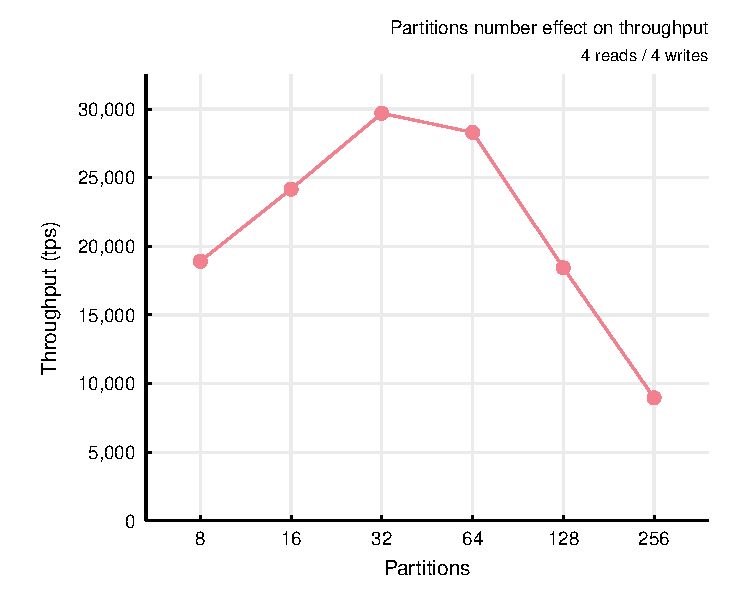
\includegraphics[width=0.5\textwidth]{figures/psi_partitions_throughput.pdf}
\vspace{-0.75cm}
\end{center}
\caption{Performance degradation of fastPSI as the number of partitions increases.}
\label{fig:fastpsi_partition_throughput}
\end{figure}
